\documentclass[12pt,a4paper]{article}

% ─── Page Layout ───────────────────────────────────────────────────────────────
\usepackage[a4paper, margin=0.8in, headheight=14pt]{geometry}

% ─── Fonts (XeLaTeX) ───────────────────────────────────────────────────────────
\usepackage{fontspec}
\usepackage{unicode-math}
\setmainfont{TeX Gyre Pagella}
\setmonofont[Scale=0.88]{TeX Gyre Cursor}
\setmathfont{Latin Modern Math}

% ─── Packages ──────────────────────────────────────────────────────────────────
\usepackage{xcolor}
\usepackage{colortbl}
\usepackage{titlesec}
\usepackage{enumitem}
\usepackage{tabularx}
\usepackage{booktabs}
\usepackage{array}
\usepackage{amsmath}
\usepackage{tikz}
\usetikzlibrary{shapes.geometric, arrows.meta, positioning, calc, fit, decorations.pathreplacing}
\usepackage{tcolorbox}
\tcbuselibrary{skins, breakable}
\usepackage{hyperref}
\usepackage{fancyhdr}
\usepackage{graphicx}
\usepackage{microtype}
\hyphenpenalty=10000
\exhyphenpenalty=10000
\sloppy
\usepackage{caption}
\usepackage{setspace}
\usepackage{multirow}
\usepackage{tocloft}

% ─── Q&A helper ────────────────────────────────────────────────────────────────
\newcommand{\Q}[1]{\textbf{#1}\par\noindent\ignorespaces}

% ─── Colour Palette ────────────────────────────────────────────────────────────
\definecolor{myred}{RGB}{196,30,58}
\definecolor{mydark}{RGB}{30,30,50}
\definecolor{mygreen}{RGB}{14,120,80}
\definecolor{myteal}{RGB}{0,130,140}
\definecolor{myamber}{RGB}{180,100,0}
\definecolor{mypurple}{RGB}{100,30,160}
\definecolor{mygray}{RGB}{246,247,249}
\definecolor{mgframe}{RGB}{180,185,200}
\definecolor{watermark}{RGB}{145,150,170}
\definecolor{hdrred}{RGB}{250,232,235}
\definecolor{hdrgreen}{RGB}{220,244,233}
\definecolor{hdrteal}{RGB}{220,242,244}
\definecolor{hdramber}{RGB}{253,242,215}
\definecolor{hdrpurple}{RGB}{238,228,255}
\definecolor{hdrgray}{RGB}{238,240,245}
\definecolor{rowalt}{RGB}{250,251,253}

% ─── Section Formatting ────────────────────────────────────────────────────────
\titleformat{\section}
  {\large\bfseries\color{myred}}{\thesection.}{0.5em}{}
  [\vspace{1pt}{\color{myred}\rule{\linewidth}{0.8pt}}]
\titleformat{\subsection}
  {\normalsize\bfseries\color{myteal}}{\thesubsection}{0.5em}{}
\titlespacing*{\section}{0pt}{18pt}{7pt}
\titlespacing*{\subsection}{0pt}{11pt}{4pt}

% ─── Paragraph ─────────────────────────────────────────────────────────────────
\setlength{\parindent}{0pt}
\setlength{\parskip}{4pt}

% ─── TOC Styling ───────────────────────────────────────────────────────────────
\renewcommand{\cfttoctitlefont}{\large\bfseries\color{myred}}
\renewcommand{\cftaftertoctitle}{\par\noindent{\color{myred}\rule{\linewidth}{0.8pt}}}
\setlength{\cftbeforetoctitleskip}{0pt}
\setlength{\cftaftertoctitleskip}{6pt}
\renewcommand{\cftsecfont}{\normalsize\bfseries\color{mydark}}
\renewcommand{\cftsecpagefont}{\normalsize\bfseries\color{mydark}}
\renewcommand{\cftsecleader}{\cftdotfill{\cftdotsep}}
\setlength{\cftbeforesecskip}{7pt}
\renewcommand{\cftsubsecfont}{\small\color{mydark}}
\renewcommand{\cftsubsecpagefont}{\small\color{mydark}}
\setlength{\cftbeforesubsecskip}{3pt}
\setlength{\cftsubsecindent}{1.4em}

% ─── Table helpers ─────────────────────────────────────────────────────────────
\renewcommand{\arraystretch}{1.45}
\setlength{\tabcolsep}{6pt}
\arrayrulecolor{mydark}
\newcolumntype{B}[1]{>{\small\bfseries\raggedright\arraybackslash}m{#1}}
\newcolumntype{Y}{>{\small\raggedright\arraybackslash}X}
\renewcommand{\tabularxcolumn}[1]{m{#1}}

% ─── Header / Footer ───────────────────────────────────────────────────────────
\pagestyle{fancy}
\fancyhf{}
\fancyhead[L]{\small\color{myred}\textbf{PE-EC603B}\;\color{mydark}--- Bio-Medical Electronics}
\fancyhead[R]{\small\color{myteal}\textbf{Module 4 Notes}}
\fancyfoot[C]{\small\color{mydark}\thepage}
\fancyfoot[R]{\small\color{watermark}\textit{\copyright\ Biraj}}
\renewcommand{\headrulewidth}{0.5pt}
\renewcommand{\footrulewidth}{0.3pt}

% ─── Hyperref ──────────────────────────────────────────────────────────────────
\hypersetup{
  colorlinks=true, linkcolor=myteal, urlcolor=myteal,
  pdfauthor={Biraj Sarkar},
  pdftitle={PE-EC603B --- Module 4 Notes}
}

% ─── tcolorbox styles ──────────────────────────────────────────────────────────
\tcbset{
  tikzbox/.style={
    colback=mygray, colframe=mgframe, boxrule=0.6pt, arc=4pt,
    left=8pt, right=8pt, top=6pt, bottom=6pt,
    colbacktitle=mgframe, coltitle=mydark,
    fonttitle=\small\bfseries
  },
  defbox/.style={
    colback=hdrgreen, colframe=mygreen, boxrule=0.8pt, arc=4pt,
    left=9pt, right=9pt, top=6pt, bottom=6pt,
    colbacktitle=mygreen, coltitle=white,
    fonttitle=\small\bfseries
  },
  formulabox/.style={
    colback=hdrteal, colframe=myteal, boxrule=0.8pt, arc=4pt,
    left=9pt, right=9pt, top=7pt, bottom=7pt,
    colbacktitle=myteal, coltitle=white,
    fonttitle=\small\bfseries
  },
  examplebox/.style={
    colback=hdramber, colframe=myamber, boxrule=0.8pt, arc=4pt,
    left=9pt, right=9pt, top=6pt, bottom=6pt,
    colbacktitle=myamber, coltitle=white,
    fonttitle=\small\bfseries
  },
  masonbox/.style={
    colback=hdrpurple, colframe=mypurple, boxrule=0.8pt, arc=4pt,
    left=9pt, right=9pt, top=6pt, bottom=6pt,
    colbacktitle=mypurple, coltitle=white,
    fonttitle=\small\bfseries
  },
  exambox/.style={
    colback=hdrpurple, colframe=mypurple, boxrule=1pt, arc=5pt,
    left=10pt, right=10pt, top=8pt, bottom=8pt,
    colbacktitle=mypurple, coltitle=white,
    fonttitle=\bfseries,
    breakable, title after break={\textbf{Frequently Asked / Viva Questions (contd.)}}}
}
\tcbset{breakable}

% ─── TikZ styles ───────────────────────────────────────────────────────────────
\tikzset{
  block/.style={rectangle, draw=myteal, fill=hdrteal,
    text width=2.4cm, align=center, minimum height=0.95cm,
    font=\small, rounded corners=3pt, line width=0.7pt},
  redblock/.style={rectangle, draw=myred, fill=hdrred,
    text width=2.4cm, align=center, minimum height=0.95cm,
    font=\small, rounded corners=3pt, line width=0.7pt},
  greenblock/.style={rectangle, draw=mygreen, fill=hdrgreen,
    text width=2.4cm, align=center, minimum height=0.95cm,
    font=\small, rounded corners=3pt, line width=0.7pt},
  amberblock/.style={rectangle, draw=myamber, fill=hdramber,
    text width=2.4cm, align=center, minimum height=0.95cm,
    font=\small, rounded corners=3pt, line width=0.7pt},
  purpblock/.style={rectangle, draw=mypurple, fill=hdrpurple,
    text width=2.4cm, align=center, minimum height=0.95cm,
    font=\small, rounded corners=3pt, line width=0.7pt},
  sumjunc/.style={circle, draw=myamber, fill=hdramber,
    minimum size=0.62cm, font=\small, line width=0.8pt},
  arrow/.style={-Stealth, thick, color=mydark},
  redarrow/.style={-Stealth, thick, color=myred},
  line/.style={thick, color=mydark}
}

% ═══════════════════════════════════════════════════════════════════════════════
\begin{document}
% ═══════════════════════════════════════════════════════════════════════════════

\begin{center}
  {\LARGE\bfseries\color{myred} PE-EC603B --- Bio-Medical Electronics}\\[5pt]
  {\normalsize\color{mydark} Semester VI \quad$\bullet$\quad 3L:0T:0P \quad$\bullet$\quad 3 Credits}\\[3pt]
  {\normalsize\color{myteal}\textbf{Module 4 Exam Notes: Prostheses, Therapeutic Devices and Electrical Safety}}\\[3pt]
  {\small\color{mydark} CGEC \;$|$\; B.Tech ECE (2023--27) \;$|$\; \textit{Biraj Sarkar}}
\end{center}
\vspace{2pt}
\noindent{\color{myred}\rule{\linewidth}{1.5pt}}
\vspace{2pt}

\hypersetup{linkcolor=mydark}
\tableofcontents
\hypersetup{linkcolor=myteal}
\newpage

% ===============================================================================
\section{Cardiac Pacemakers}
% ===============================================================================

\begin{tcolorbox}[defbox, title={\textbf{Definition: Cardiac Pacemaker}}]
A \textbf{cardiac pacemaker} is an implantable electronic device that delivers controlled electrical stimuli to the heart muscle to maintain an adequate heart rate when the natural conduction system (SA node, AV node) fails or is too slow (bradycardia, heart block, sick sinus syndrome).
\end{tcolorbox}

\subsection{Pacemaker Block Diagram}

\begin{tcolorbox}[tikzbox, title={Cardiac Pacemaker Block Diagram}]
\centering
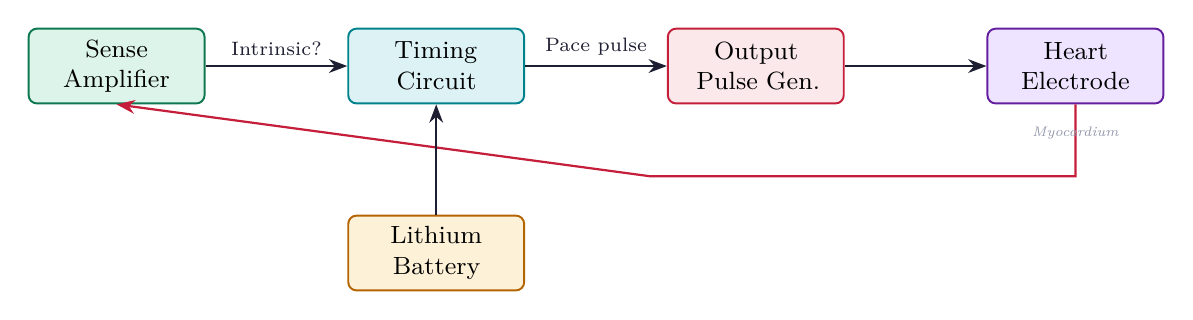
\begin{tikzpicture}[node distance=0.7cm and 1.6cm, thick, font=\small]
  % Sense
  \node[greenblock, text width=2.0cm] (sense) {Sense\\Amplifier};
  % Timing
  \node[block, text width=2.0cm, right=1.8cm of sense] (timing) {Timing\\Circuit};
  % Output
  \node[redblock, text width=2.0cm, right=1.8cm of timing] (output) {Output\\Pulse Gen.};
  % Battery
  \node[amberblock, text width=2.0cm, below=1.4cm of timing] (batt) {Lithium\\Battery};
  % Lead/electrode
  \node[purpblock, text width=2.0cm, right=1.8cm of output] (heart) {Heart\\Electrode};

  % Arrows
  \draw[arrow] (sense) -- node[above, font=\scriptsize] {Intrinsic?} (timing);
  \draw[arrow] (timing) -- node[above, font=\scriptsize] {Pace pulse} (output);
  \draw[arrow] (output) -- (heart);
  \draw[redarrow] (heart) -- ++(0,-1.4) -- ++(-5.4,0) -- (sense.south);
  \draw[arrow] (batt) -- (timing);
  \node[font=\tiny\itshape, color=watermark, below=0.15cm of heart] {Myocardium};
\end{tikzpicture}
\end{tcolorbox}

\subsection{Types of Pacemakers}

\par\noindent
\begin{tabularx}{\linewidth}{|B{2.8cm}|Y|Y|}
\hline
\textbf{Type} & \textbf{\color{myteal}Description} & \textbf{\color{mygreen}Use} \\
\hline
\textbf{Single-chamber (AAI / VVI)} & Senses and paces one chamber only (atrium or ventricle). & Sick sinus syndrome (AAI); complete heart block (VVI). \\
\hline
\textbf{Dual-chamber (DDD)} & Senses and paces both atrium and ventricle; maintains AV synchrony. & AV block with intact SA node. \\
\hline
\textbf{Rate-responsive (DDDR)} & Uses sensor (accelerometer, minute ventilation) to increase rate during exercise. & Chronotropic incompetence, active patients. \\
\hline
\textbf{CRT (Biventricular)} & Paces both ventricles simultaneously to resynchronize contraction. & Heart failure with left bundle branch block. \\
\hline
\textbf{Leadless pacemaker} & Capsule implanted directly in right ventricle; no transvenous lead. & Single-chamber pacing without lead complications. \\
\hline
\end{tabularx}

\subsection{Pacemaker Timing Parameters}

\begin{tcolorbox}[formulabox, title={\textbf{Pacemaker Timing Intervals}}]
\renewcommand{\arraystretch}{1.3}
\begin{tabularx}{\linewidth}{B{3.8cm} X}
Pacing Rate & $\text{Rate (bpm)} = \dfrac{60\,000}{\text{Pacing Interval (ms)}}$ \\[8pt]
AV Delay & Time from atrial pace/sense to ventricular pace ($\approx 120$--$200\,\text{ms}$; mimics PR interval). \\[4pt]
Refractory Period & Time after a sensed/paced event during which the pacemaker ignores signals ($\approx 250$--$400\,\text{ms}$). \\[4pt]
Escape Interval & Time from a sensed beat to the next paced beat if no intrinsic beat occurs. \\[4pt]
Pulse Width & Duration of pacing pulse ($\approx 0.4$--$1.0\,\text{ms}$). \\[4pt]
Pulse Amplitude & Voltage of pacing pulse ($\approx 2.5$--$5\,\text{V}$; must exceed stimulation threshold).
\end{tabularx}
\end{tcolorbox}

\textbf{Energy Source:} Lithium--iodide (LiI) battery; longevity $5$--$15$ years. Elective Replacement Indicator (ERI) detects end-of-battery voltage ($2.4\,\text{V}$ from $2.8\,\text{V}$ nominal).

% ===============================================================================
\section{Defibrillators}
% ===============================================================================

\begin{tcolorbox}[defbox, title={\textbf{Definition: Defibrillator}}]
A \textbf{defibrillator} is a device that delivers a controlled, high-energy electrical shock to the heart to terminate life-threatening arrhythmias such as \textbf{ventricular fibrillation (VF)} and \textbf{ventricular tachycardia (VT)}, depolarizing all cardiac cells simultaneously so that the SA node can resume normal pacemaker control.
\end{tcolorbox}

\subsection{Principle and Types}

\textbf{Ventricular fibrillation} is chaotic, uncoordinated cardiac electrical activity --- the heart quivers rather than pumping. Without defibrillation within $\approx 4$--$6\,\text{minutes}$, brain death ensues.

\par\noindent
\begin{tabularx}{\linewidth}{|B{3.0cm}|Y|Y|}
\hline
\textbf{Type} & \textbf{\color{myteal}Description} & \textbf{\color{mygreen}Energy} \\
\hline
\textbf{External} & Paddle or adhesive pad electrodes on chest wall. & 150--360 J (monophasic); 120--200 J (biphasic). \\
\hline
\textbf{Internal} & Used during cardiac surgery; paddles placed directly on heart. & 20--50 J. \\
\hline
\textbf{ICD (Implantable Cardioverter Defibrillator)} & Permanently implanted; monitors rhythm continuously; delivers therapy automatically. & 25--40 J; also provides anti-tachycardia pacing. \\
\hline
\textbf{AED (Automated External Defibrillator)} & Portable; analyses rhythm and advises/delivers shock automatically. Designed for lay-rescuer use. & 120--200 J (biphasic). \\
\hline
\end{tabularx}

\subsection{Defibrillator Circuit and Waveforms}

\begin{tcolorbox}[tikzbox, title={Defibrillator Discharge Circuit and Waveforms}]
\centering
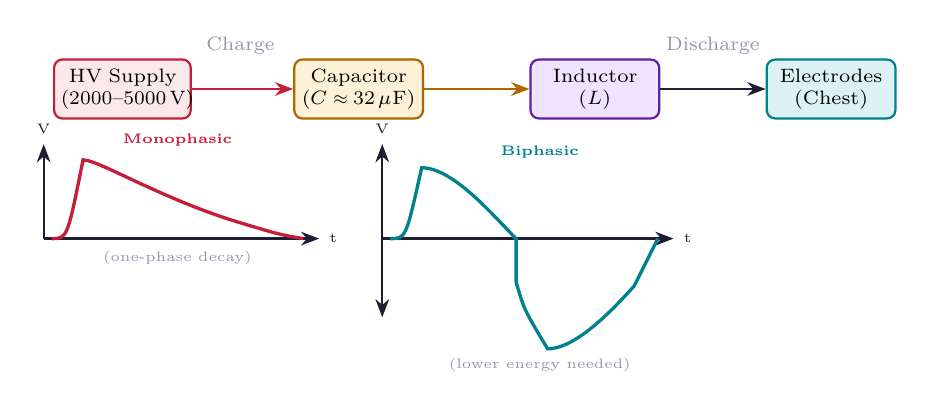
\begin{tikzpicture}[thick, font=\small]
  % --- Circuit ---
  % Capacitor charging from high-voltage supply
  \node[draw=myred, fill=hdrred, rounded corners=3pt,
        minimum width=1.6cm, minimum height=0.7cm, font=\scriptsize,
        align=center, text width=1.5cm] (hv) at (-4.5, 2.0) {HV Supply\\{\scriptsize(2000--5000\,V)}};
  \node[draw=myamber, fill=hdramber, rounded corners=3pt,
        minimum width=1.4cm, minimum height=0.7cm, font=\scriptsize,
        align=center, text width=1.4cm] (cap) at (-1.5, 2.0) {Capacitor\\{\scriptsize($C \approx 32\,\mu\text{F}$)}};
  \node[draw=mypurple, fill=hdrpurple, rounded corners=3pt,
        minimum width=1.4cm, minimum height=0.7cm, font=\scriptsize,
        align=center, text width=1.4cm] (ind) at (1.5, 2.0) {Inductor\\($L$)};
  \node[draw=myteal, fill=hdrteal, rounded corners=3pt,
        minimum width=1.4cm, minimum height=0.7cm, font=\scriptsize,
        align=center, text width=1.4cm] (pad) at (4.5, 2.0) {Electrodes\\{\scriptsize(Chest)}};

  \draw[arrow, color=myred] (hv) -- (cap);
  \draw[arrow, color=myamber] (cap) -- (ind);
  \draw[arrow] (ind) -- (pad);

  \node[font=\scriptsize, color=watermark] at (-3.0, 2.55) {Charge};
  \node[font=\scriptsize, color=watermark] at (3.0, 2.55) {Discharge};

  % --- Waveform comparison ---
  \begin{scope}[yshift=-0.4cm]
    % Monophasic axis
    \draw[arrow] (-5.5, 0.5) -- (-2.0, 0.5) node[right, font=\tiny] {t};
    \draw[arrow] (-5.5, 0.5) -- (-5.5, 1.7) node[above, font=\tiny] {V};
    \draw[color=myred, line width=1.2pt] (-5.4, 0.5)
      .. controls (-5.2,0.5) .. (-5.0, 1.5)
      .. controls (-4.8,1.5) and (-4.0, 1.0) .. (-3.0, 0.7)
      .. controls (-2.5, 0.55) .. (-2.2, 0.5);
    \node[font=\tiny\bfseries, color=myred] at (-3.8, 1.75) {Monophasic};
    \node[font=\tiny, color=watermark] at (-3.8, 0.25) {(one-phase decay)};

    % Biphasic axis
    \draw[arrow] (-1.2, 0.5) -- (2.5, 0.5) node[right, font=\tiny] {t};
    \draw[arrow] (-1.2, 0.5) -- (-1.2, 1.7) node[above, font=\tiny] {V};
    \draw[arrow] (-1.2, 0.5) -- (-1.2, -0.5);
    \draw[color=myteal, line width=1.2pt] (-1.1, 0.5)
      .. controls (-0.9, 0.5) .. (-0.7, 1.4)
      .. controls (-0.3, 1.4) and (0.2, 0.8) .. (0.5, 0.5)
      -- (0.5, -0.05)
      .. controls (0.6, -0.4) .. (0.9, -0.9)
      .. controls (1.2, -0.9) and (1.6, -0.55) .. (2.0, -0.1)
      -- (2.3, 0.5);
    \node[font=\tiny\bfseries, color=myteal] at (0.8, 1.6) {Biphasic};
    \node[font=\tiny, color=watermark] at (0.8, -1.1) {(lower energy needed)};
  \end{scope}
\end{tikzpicture}
\end{tcolorbox}

\textbf{Energy stored in capacitor:} $E = \dfrac{1}{2}CV^2$. For $C = 32\,\mu\text{F}$ and $V = 3000\,\text{V}$: $E = \dfrac{1}{2}\times 32\times10^{-6}\times(3000)^2 = 144\,\text{J}$.

\textbf{Biphasic vs.\ Monophasic:} Biphasic waveforms reverse polarity partway through the shock. They are more effective at lower energies ($\approx 150$--$200\,\text{J}$ vs.\ $360\,\text{J}$) and cause less myocardial injury. All modern defibrillators use biphasic waveforms.

% ===============================================================================
\section{Heart-Lung Machine (Cardiopulmonary Bypass)}
% ===============================================================================

\begin{tcolorbox}[defbox, title={\textbf{Heart-Lung Machine}}]
The \textbf{heart-lung machine} (cardiopulmonary bypass pump, CPB) temporarily takes over the function of the heart and lungs during open-heart surgery. It oxygenates blood, removes carbon dioxide, and pumps it back to the body, allowing surgeons to operate on a still, bloodless heart.
\end{tcolorbox}

\subsection{Components and Operation}

\begin{tcolorbox}[tikzbox, title={Cardiopulmonary Bypass Circuit}]
\centering
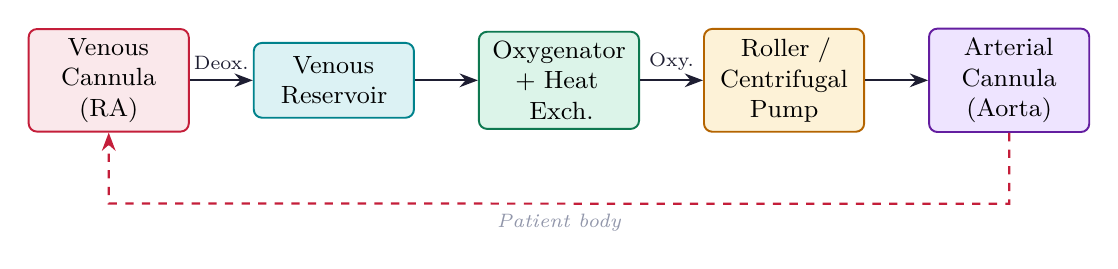
\begin{tikzpicture}[
  node distance=0.8cm and 0.8cm, thick, font=\small,
  sredblock/.style={rectangle, draw=myred, fill=hdrred, text width=1.8cm, align=center, minimum height=0.95cm, rounded corners=3pt, line width=0.7pt},
  sblock/.style={rectangle, draw=myteal, fill=hdrteal, text width=1.8cm, align=center, minimum height=0.95cm, rounded corners=3pt, line width=0.7pt},
  sgreenblock/.style={rectangle, draw=mygreen, fill=hdrgreen, text width=1.8cm, align=center, minimum height=0.95cm, rounded corners=3pt, line width=0.7pt},
  samberblock/.style={rectangle, draw=myamber, fill=hdramber, text width=1.8cm, align=center, minimum height=0.95cm, rounded corners=3pt, line width=0.7pt},
  spurpblock/.style={rectangle, draw=mypurple, fill=hdrpurple, text width=1.8cm, align=center, minimum height=0.95cm, rounded corners=3pt, line width=0.7pt}
]
  % Nodes
  \node[sredblock] (ra) {Venous\\Cannula\\(RA)};
  \node[sblock, right=0.8cm of ra] (resvr) {Venous\\Reservoir};
  \node[sgreenblock, right=0.8cm of resvr] (oxyg) {Oxygenator\\+ Heat Exch.};
  \node[samberblock, right=0.8cm of oxyg] (pump) {Roller /\\Centrifugal\\Pump};
  \node[spurpblock, right=0.8cm of pump] (ao) {Arterial\\Cannula\\(Aorta)};

  % Arrows
  \draw[arrow] (ra) -- node[above, font=\scriptsize] {Deox.} (resvr);
  \draw[arrow] (resvr) -- (oxyg);
  \draw[arrow] (oxyg) -- node[above, font=\scriptsize] {Oxy.} (pump);
  \draw[arrow] (pump) -- (ao);

  % Body loop at bottom
  \draw[redarrow, dashed] (ao.south) -- ++(0,-0.9) -- ($(ra.south)+(0,-0.9)$) node[midway, below, font=\scriptsize\itshape, color=watermark] {Patient body} -- (ra.south);
\end{tikzpicture}
\end{tcolorbox}

\textbf{Key components:}
\begin{itemize}[leftmargin=*, itemsep=3pt]
  \item \textbf{Oxygenator (Membrane type):} Blood flows past a semipermeable membrane; O$_2$ diffuses in and CO$_2$ diffuses out. Replaces the lungs.
  \item \textbf{Roller Pump / Centrifugal Pump:} Provides non-pulsatile (roller) or pulsatile (centrifugal) blood flow. Replaces the heart.
  \item \textbf{Heat Exchanger:} Lowers body temperature (hypothermia, $28$--$32\,^{\circ}$C) during surgery to reduce metabolic demand; rewarms blood before weaning from bypass.
  \item \textbf{Arterial Filter:} Removes air bubbles and particulate emboli from the arterial return line.
  \item \textbf{Cardioplegia system:} Cold potassium-rich solution delivered to coronary arteries to arrest the heart in diastole (electromechanical quiescence).
\end{itemize}

% ===============================================================================
\section{Artificial Kidney (Dialysis)}
% ===============================================================================

\begin{tcolorbox}[defbox, title={\textbf{Haemodialysis (Artificial Kidney)}}]
\textbf{Haemodialysis} is a renal replacement therapy for patients with End-Stage Renal Disease (ESRD). Blood is withdrawn, passed through a \textbf{dialyser} (artificial kidney) containing a semipermeable membrane, and returned to the body. The dialyser removes metabolic waste products (urea, creatinine, excess electrolytes) and excess water by the processes of \textbf{diffusion} and \textbf{ultrafiltration}.
\end{tcolorbox}

\subsection{Principles of Dialysis}

\begin{tcolorbox}[formulabox, title={\textbf{Mass Transport Mechanisms in Haemodialysis}}]
\renewcommand{\arraystretch}{1.3}
\begin{tabularx}{\linewidth}{B{3.2cm} X}
Diffusion & Movement of solutes across membrane from high to low concentration. Main mechanism for small solutes (urea, creatinine, potassium). \\[4pt]
Ultrafiltration & Hydraulic pressure drives water (and dissolved solutes) across the membrane. Controlled to remove excess fluid ($1$--$3\,\text{L/session}$). \\[4pt]
Clearance ($K$) & $K = \dfrac{Q_{Bi} \cdot C_{Bi} - Q_{Bo} \cdot C_{Bo}}{C_{Bi}}$ \quad (mL/min) \\[8pt]
KT/V & Urea dialysis adequacy measure: $Kt/V = -\ln(R - 0.008t) + (4-3.5R)\times\dfrac{UF}{W}$ \quad target $\geq 1.2$.
\end{tabularx}
\end{tcolorbox}

\subsection{Haemodialysis Circuit}

Blood is withdrawn from a vascular access (arteriovenous fistula, graft, or central venous catheter), anticoagulated with heparin, pumped through the dialyser at $200$--$500\,\text{mL/min}$ and returned. The dialysate (purified water + electrolytes) flows counter-current to blood at $500$--$800\,\text{mL/min}$.

\textbf{Safety alarms in a dialysis machine:}
\begin{itemize}[leftmargin=*, itemsep=2pt]
  \item Air bubble detector (ultrasonic).
  \item Venous pressure monitor (clot detection).
  \item Blood leak detector (photometric --- detects red blood cells in dialysate).
  \item Conductivity monitor (ensures correct dialysate concentration).
  \item Temperature alarm ($\pm 1\,^{\circ}$C from $37\,^{\circ}$C).
\end{itemize}

\textbf{Peritoneal Dialysis (PD):} Dialysate is instilled into the peritoneal (abdominal) cavity; the peritoneal membrane acts as the dialyser. No blood circuit required; performed at home. Less efficient than haemodialysis but better for residual renal function preservation.

% ===============================================================================
\section{Aids for the Handicapped}
% ===============================================================================

\subsection{Cochlear Implant}

\begin{tcolorbox}[defbox, title={\textbf{Cochlear Implant}}]
A \textbf{cochlear implant} is an electronic device that bypasses damaged hair cells in the cochlea and directly stimulates the auditory nerve fibres with electrical impulses, enabling profoundly deaf or severely hard-of-hearing individuals to perceive sound.
\end{tcolorbox}

\textbf{Components:}
\begin{enumerate}[leftmargin=*, itemsep=3pt]
  \item \textbf{Microphone} --- picks up sound from environment.
  \item \textbf{Speech Processor} (external, worn behind the ear) --- digitizes and filters sound into frequency bands; encodes into stimulation commands.
  \item \textbf{Transmitter Coil} (external) --- sends encoded signals transcutaneously via radiofrequency link to the internal receiver.
  \item \textbf{Internal Receiver/Stimulator} (implanted under skin) --- decodes RF signal, generates electrical pulses.
  \item \textbf{Electrode Array} (implanted in cochlea) --- 12--22 electrodes arranged tonotopically; each electrode stimulates a different frequency region of the auditory nerve.
\end{enumerate}

\subsection{Prosthetic Limbs}

\par\noindent
\begin{tabularx}{\linewidth}{|B{2.8cm}|Y|Y|}
\hline
\textbf{Type} & \textbf{\color{myteal}Control Mechanism} & \textbf{\color{mygreen}Application} \\
\hline
\textbf{Passive prosthesis} & Cosmetic only; no powered movement. & Upper/lower limb amputation cosmetic restoration. \\
\hline
\textbf{Body-powered} & Harness and cable system; shoulder/elbow movement activates hook or hand. & Upper limb; robust, low cost, proprioceptive feedback. \\
\hline
\textbf{Myoelectric (EMG-controlled)} & Surface EMG from residual muscles controls motor-driven hand/elbow. & Upper limb; intuitive control; electrically powered. \\
\hline
\textbf{Microprocessor knee} & Sensors and microcontroller adjust damping in real time for variable gait. & Trans-femoral (above-knee) amputation. \\
\hline
\end{tabularx}

\subsection{Other Assistive Devices}

\begin{itemize}[leftmargin=*, itemsep=3pt]
  \item \textbf{Visual prosthesis (Bionic eye):} Electrode array on retina or visual cortex stimulated by camera-processed signals to restore partial vision.
  \item \textbf{Deep Brain Stimulator (DBS):} Electrodes implanted in subthalamic nucleus; high-frequency ($130$--$180\,\text{Hz}$) electrical stimulation treats Parkinson's disease tremor.
  \item \textbf{Functional Electrical Stimulation (FES):} External electrodes stimulate paralysed muscles in paraplegic patients for assisted hand grasp or standing.
  \item \textbf{Hearing Aid:} Amplifies sound; does not bypass cochlea (unlike cochlear implant). Uses Class D amplifiers; ITE (in-the-ear) or BTE (behind-the-ear) form factors.
\end{itemize}

% ===============================================================================
\section{Electrical Safety in Medical Environments}
% ===============================================================================

\begin{tcolorbox}[defbox, title={\textbf{Importance of Electrical Safety}}]
Medical instruments are directly connected to or in close contact with patients. Even small leakage currents that are harmless in everyday life can be lethal in medical situations where electrodes bypass skin resistance or are in contact with the heart. Electrical safety standards (IEC 60601) define acceptable limits to protect both patients and operators.
\end{tcolorbox}

\subsection{Macroshock and Microshock}

\begin{tcolorbox}[formulabox, title={\textbf{Electric Shock Thresholds}}]
\renewcommand{\arraystretch}{1.35}
\begin{tabularx}{\linewidth}{B{3.2cm} X}
\textbf{Macroshock} & Current entering through skin. Skin resistance ($\approx 10$\,k$\Omega$--$1$\,M$\Omega$ dry) limits current. \\[4pt]
Perception threshold & $\approx 1\,\text{mA}$ (50 Hz AC). \\[4pt]
Let-go threshold & $\approx 10$--$20\,\text{mA}$ (muscle tetany; cannot release conductor). \\[4pt]
Ventricular fibrillation & $\approx 100\,\text{mA}$ (chest surface current). \\[4pt]
Cardiac arrest / Burns & $\approx 1$--$10\,\text{A}$. \\[6pt]
\textbf{Microshock} & Current applied directly to heart (via catheter, pacemaker leads). Skin resistance bypassed. \\[4pt]
VF threshold (intracardiac) & As low as $\mathbf{10\text{--}50\,\mu\text{A}}$ (cardiac catheter, pacemaker wire). \\[4pt]
IEC 60601 limit (patient leakage) & $\leq 10\,\mu\text{A}$ (Type CF equipment connected to heart).
\end{tabularx}
\end{tcolorbox}

\subsection{Sources of Leakage Current}

\begin{itemize}[leftmargin=*, itemsep=3pt]
  \item \textbf{Capacitive leakage:} Power line coupling through stray capacitance between mains wiring and equipment chassis.
  \item \textbf{Resistive leakage:} Insulation degradation due to aging, moisture, or damage.
  \item \textbf{Inductive leakage:} Magnetic coupling from transformers or motors.
\end{itemize}

\subsection{Safety Methods and Standards}

\par\noindent
\begin{tabularx}{\linewidth}{|B{3.0cm}|Y|}
\hline
\textbf{Protection Method} & \textbf{Description} \\
\hline
\textbf{Earth (Ground) connection} & Chassis connected to protective earth; fault current diverted away from patient. \\
\hline
\textbf{Double insulation} & Two separate insulation layers between mains and chassis; no earth required. \\
\hline
\textbf{Galvanic isolation} & Patient circuit isolated from mains via transformer, optocouplers, or RF links; leakage path broken. \\
\hline
\textbf{Right-Leg Drive (ECG)} & Driven shield reduces common-mode interference; active cancellation of body surface potentials. \\
\hline
\textbf{Equipotential bonding} & All metal surfaces in the patient's area bonded to a common potential to eliminate voltage differences. \\
\hline
\textbf{GFCI / RCD} & Ground Fault Circuit Interrupter detects mains leakage $> 5\,\text{mA}$ and trips the supply. \\
\hline
\end{tabularx}

\subsection{IEC 60601 Equipment Classification}

\par\noindent
\begin{tabularx}{\linewidth}{|B{2.0cm}|Y|>{\centering\arraybackslash}m{2.8cm}|}
\hline
\textbf{Class} & \textbf{Description} & \textbf{Max.\ Patient Leakage} \\
\hline
\textbf{Type B} & General body contact; not directly connected to heart. & $100\,\mu\text{A}$ \\
\hline
\textbf{Type BF} & Floating (isolated) patient connection; body contact. & $100\,\mu\text{A}$ (isolated) \\
\hline
\textbf{Type CF} & Directly connected to heart (e.g., intracardiac catheter). & $10\,\mu\text{A}$ \\
\hline
\end{tabularx}

\newpage
% ===============================================================================
% MANDATORY QUICK REVISION PAGE
% ===============================================================================
\begin{center}
  {\large\bfseries\color{myred} Quick Revision --- Module 4}\\[3pt]
  {\small\color{mydark} Prostheses, Therapeutic Devices and Electrical Safety $|$ PE-EC603B}
\end{center}
\noindent{\color{myred}\rule{\linewidth}{1.2pt}}
\vspace{4pt}

\begin{tcolorbox}[formulabox, title={\textbf{Key Formulas and Thresholds}}]
\renewcommand{\arraystretch}{1.3}
\begin{tabularx}{\linewidth}{B{4.2cm} X}
Pacemaker rate & $\text{Rate} = 60000 / \text{interval(ms)}$ \\[4pt]
Defibrillator energy & $E = \dfrac{1}{2}CV^2$ \quad (J) \\[8pt]
Dialysis adequacy & $Kt/V \geq 1.2$ for adequate haemodialysis \\[4pt]
Macroshock VF & $\approx 100\,\text{mA}$ (skin current, 50 Hz) \\[4pt]
Microshock VF & $\approx 10$--$50\,\mu\text{A}$ (intracardiac) \\[4pt]
IEC CF leakage limit & $\leq 10\,\mu\text{A}$ (direct cardiac contact) \\[4pt]
IEC B/BF leakage limit & $\leq 100\,\mu\text{A}$
\end{tabularx}
\end{tcolorbox}

\begin{tcolorbox}[defbox, title={\textbf{One-Line Definitions}}]
\begin{itemize}[leftmargin=*, itemsep=2.5pt, topsep=0pt]
  \item \textbf{Pacemaker:} Implantable device delivering timed electrical pulses to maintain adequate heart rate.
  \item \textbf{Defibrillator:} Device delivering high-energy shock to terminate VF/VT by simultaneous depolarization of all cardiac cells.
  \item \textbf{AED:} Automated External Defibrillator; public-access defibrillator that analyses rhythm and advises shock delivery.
  \item \textbf{ICD:} Implantable Cardioverter Defibrillator; automatic implantable device sensing and treating VF/VT.
  \item \textbf{Heart-Lung Machine:} Cardiopulmonary bypass device replacing heart and lung function during open-heart surgery.
  \item \textbf{Haemodialysis:} Extracorporeal blood purification via diffusion through semipermeable membrane for renal failure.
  \item \textbf{Ultrafiltration:} Pressure-driven removal of water across a dialysis membrane.
  \item \textbf{Cochlear Implant:} Electronic device directly stimulating auditory nerve fibres to restore hearing in profound deafness.
  \item \textbf{Macroshock:} Dangerous electrical current entering body through skin ($> 100\,\text{mA}$ causes VF).
  \item \textbf{Microshock:} Tiny current ($10$--$50\,\mu\text{A}$) directly reaching the heart via catheter/pacemaker wire; causes VF.
  \item \textbf{Galvanic Isolation:} Breaking the electrical connection between mains and patient circuit to eliminate leakage path.
\end{itemize}
\end{tcolorbox}

\begin{tcolorbox}[exambox, title={\textbf{Frequently Asked / Viva Questions}}]
\begin{enumerate}[topsep=0pt, label=\textbf{Q\arabic*.}, itemsep=5pt]
  \item \Q{What is a cardiac pacemaker? When is it indicated?}
    A pacemaker is an implanted electronic device delivering controlled electrical stimuli to the heart to maintain an adequate rate. It is indicated in bradycardia, sick sinus syndrome, complete (3rd degree) AV block, and heart failure (CRT).
  \item \Q{What are the modes of a DDD pacemaker?}
    DDD: first D = paces both chambers (atrium + ventricle); second D = senses both; third D = dual response (inhibited if intrinsic beat sensed, triggered if not). It maintains AV synchrony, mimicking natural conduction.
  \item \Q{What is the difference between a pacemaker and a defibrillator?}
    A pacemaker delivers low-energy ($< 5\,\text{V}$, $0.4$--$1\,\text{ms}$) pulses repeatedly to sustain a minimum heart rate (treats \textit{too slow}). A defibrillator delivers a single high-energy shock ($120$--$360\,\text{J}$) to terminate fibrillation (treats \textit{chaotic fast}). An ICD combines both functions.
  \item \Q{Why are biphasic defibrillation waveforms preferred over monophasic?}
    Biphasic waveforms reverse polarity partway through discharge. This ``tidies up'' residual charge-related effects on cell membranes, achieving the same defibrillation threshold at $\approx 40\%$ lower energy, reducing post-shock myocardial injury compared to monophasic waveforms.
  \item \Q{Explain the working of a heart-lung machine during open-heart surgery.}
    Venous blood is drained from the right atrium into a reservoir, passed through a membrane oxygenator (adds O$_2$, removes CO$_2$) and a heat exchanger (induces hypothermia to reduce metabolic demand), then pumped back into the aorta. The heart is stopped with cold cardioplegia, allowing surgery on a bloodless, still field.
  \item \Q{What is haemodialysis? Explain diffusion and ultrafiltration.}
    Haemodialysis removes metabolic waste from blood by passing it through a dialyser. \textit{Diffusion}: small solutes (urea, creatinine, K$^+$) move down their concentration gradient across the semipermeable membrane into dialysate. \textit{Ultrafiltration}: transmembrane pressure removes excess water from blood.
  \item \Q{How does a cochlear implant differ from a conventional hearing aid?}
    A hearing aid only amplifies sound; it requires residual functional hair cells in the cochlea. A cochlear implant completely bypasses the damaged cochlea and directly stimulates auditory nerve fibres with electrical pulses, providing hearing even in profound/total deafness where no hair cells survive.
  \item \Q{Define macroshock and microshock. Give the VF threshold for each.}
    \textit{Macroshock}: current entering through intact skin ($> 100\,\text{mA}$ at 50 Hz causes VF). Skin resistance ($10\,\text{k}\Omega$ to $1\,\text{M}\Omega$ dry) limits the current. \textit{Microshock}: current reaching heart directly via catheter or pacemaker lead; VF threshold as low as $10$--$50\,\mu\text{A}$ (skin resistance bypassed).
  \item \Q{What is galvanic isolation and why is it essential in medical equipment?}
    Galvanic isolation electrically separates the patient circuit from the mains supply using a transformer, optocoupler, or RF link. Any fault current or leakage from the mains cannot reach the patient, preventing both macroshock and microshock. IEC 60601 Type CF equipment must have $\leq 10\,\mu\text{A}$ patient leakage.
  \item \Q{What is an ICD? How does it detect and treat ventricular fibrillation?}
    An Implantable Cardioverter Defibrillator continuously monitors the cardiac electrogram via a right ventricular lead. On detecting VF (rate $> 200\,\text{bpm}$ with disorganized waveform), it charges an internal capacitor and delivers a shock ($25$--$40\,\text{J}$) within $10$--$20\,\text{s}$. It also provides anti-tachycardia pacing for slower VT to avoid a shock.
  \item \Q{What is functional electrical stimulation (FES)?}
    FES applies controlled electrical pulses to surface or implanted electrodes over paralysed muscles in spinal cord injury patients. By selecting the stimulation sequence, it can activate leg muscles for assisted walking, hand muscles for grasp, or respiratory muscles for diaphragmatic pacing.
\end{enumerate}
\end{tcolorbox}

\begin{tcolorbox}[tikzbox, title={Therapeutic Device Comparison}]
\renewcommand{\arraystretch}{1.4}
\par\noindent
\begin{tabularx}{\linewidth}{|B{2.8cm}|>{\centering\arraybackslash}m{2.6cm}|>{\centering\arraybackslash}m{2.6cm}|Y|}
\hline
\textbf{Device} & \textbf{\color{myred}Energy Delivered} & \textbf{\color{myteal}Purpose} & \textbf{Indication} \\
\hline
Pacemaker & $< 5$ V, $< 1$ ms pulses & Maintain heart rate & Bradycardia, AV block \\
\hline
ICD & 25--40 J shock & Terminate VF/VT & VF, VT, SCD prevention \\
\hline
External defibrillator & 120--360 J shock & Terminate VF & Cardiac arrest (VF) \\
\hline
CRT (BiV pacing) & Same as pacemaker & Resynchronize LV & Heart failure, LBBB \\
\hline
Dialysis machine & None (physical) & Remove waste, fluid & ESRD, acute renal failure \\
\hline
Heart-lung machine & Mechanical pump & Bypass heart/lungs & Open-heart surgery \\
\hline
\end{tabularx}
\end{tcolorbox}

\end{document}
